\documentclass{article}
\usepackage[utf8]{inputenc}
\usepackage[T1]{fontenc}              
\usepackage[french]{babel}
\usepackage[a4paper, margin=3cm]{geometry}
\usepackage{amsmath, amssymb, graphicx, xcolor, hyperref}
\usepackage{booktabs}


\begin{document}

\title{Rapport TNL}
\author{Amaury JACOB-PIACENTINI
\and Sharaine MALAVIJY}
\date{\today}

\maketitle

\tableofcontents
\newpage


\section{Introduction}

Le but de ce projet est de classifier des textes afin de pouvoir nous former aux divers outils de traitement du langage naturel. Pour cela, nous avons deux jeux de données différents : un jeu de données contenant des critiques de films, et un autre contenant des discours de Jaques Chirac et de François Mitterrand.\\
Nous avons divisé notre travail en plusieurs parties. Dans un premier temps, nous avons fait de l'analyse des données et du pré traitement des données. Ensuite nous avons pu commencer le travail de classification. Nous avons exploré plusieurs techniques de classification vu lors des TME et du cours.


\section{Analyse des données}
\subsection{Classification de sentiments}

\subsubsection{Description du jeu de données}

Ce jeu de données contient des critiques de films. C'est un jeu de données équilibré, nous avons 2000 critiques de films au total dont 1000 critiques positives et 1000 critiques négatives. Chaque critique de film est constituée de plusieurs phrases. Nous avons également les labels associés à chaque critique de film : 1 pour les critiques positives et 0 pour les critiques négatives.

\subsubsection{Analyse du jeu de données}

Dans un premier temps, nous avons calculer la taille du vocabulaire du jeu de données. Nous avons 39659 mots différents avant de faire un pré traitement des données.\\
Après calculer la taille du vocabulaire, il a fallu regarder la fréquence des mots dans le dataset. \\
Voici un exemple de la fréquence des mots dans le dataset : 

        \begin{table}[h]
        \centering
        \begin{tabular}{lr}
        \toprule
        Mot & Fréquence \\
        \midrule
        the & 76529 \\
        and & 35576 \\
        of & 34123 \\
        to & 31937 \\
        is & 25195 \\
        \bottomrule
        \end{tabular}
        \caption{Mots les plus fréquents (0)}
        \end{table}

Comme attendu, avant toute forme de pré traitement, les mots les plus fréquents sont les stops words.\\
Une meilleure façon de visualiser la fréquence des mots est d'utiliser un word cloud. Ainsi que la distribution de Zipf.


        \begin{figure}[h!]
            \centering
            \begin{minipage}{0.4\textwidth}
                \centering
                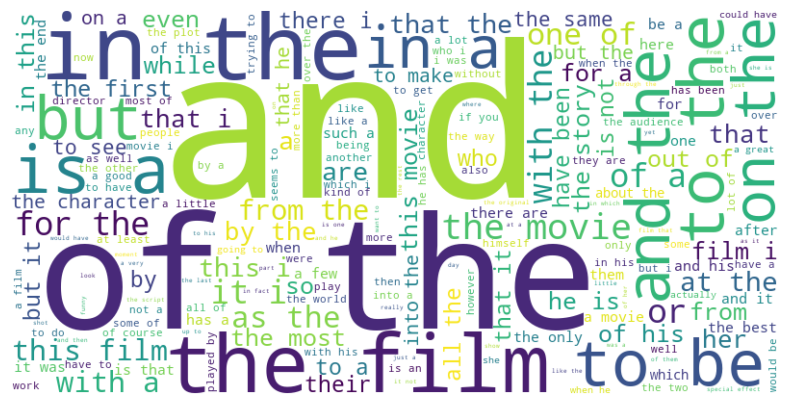
\includegraphics[width=\linewidth]{image/analyse_data/wordcloud.png}
                \caption*{\small Word cloud des critiques de films}
            \end{minipage}\hfill
            \begin{minipage}{0.4\textwidth}
                \centering
                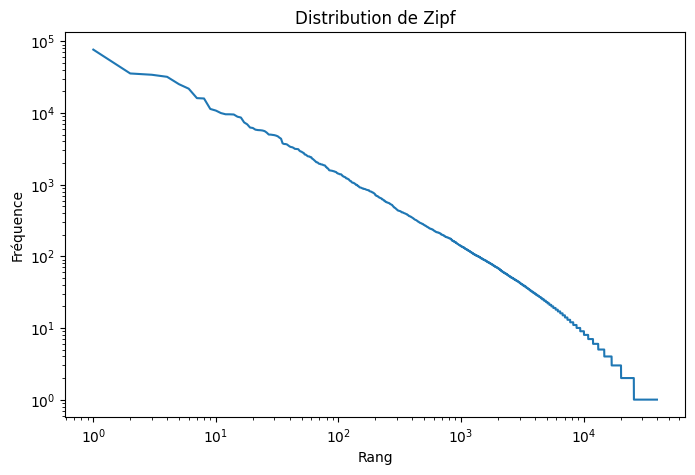
\includegraphics[width=\linewidth]{image/analyse_data/plot_zipf_film_non_pre.png}
                \caption*{\small Distribution de Zipf des critiques de films}
            \end{minipage}\hfill
            \label{fig:images-tests}
        \end{figure}

Il est aussi intéressant de regarder les mots les plus discriminants pour les critiques positives et négatives. Les mots les plus discriminants seront fait après le pré traitement des données.\\
Sur la distribution de Zipf on remarque que quelques mots sont très fréquents et que la grande majorité des mots sont peu fréquents.\\


\subsection{Classification des discours de Présidents}
\subsubsection{Description du jeu de données}

Ce jeu de données contient des discours de Jaques Chirac et de François Mitterrand. Ce jeu de données est largement plus complexe à traiter que le jeu de données de critiques de films car le jeux est largement plus désiquilibré. Nous avons 57413 phrases au total dont 49890 $(86.90\%)$ de Jaques Chirac et 7523 $(13.10\%)$ de François Mitterrand.\\
Chaque phrase est constituée de plusieurs mots. Nous avons également les labels associés à chaque phrase : 0 pour les phrases de Jaques Chirac et 1 pour les phrases de François Mitterrand.

\subsubsection{Analyse du jeu de données}
Comme dans la section précédente il a fallu calculer le nombre de mots différents présents dans le dataset. Il y 27055 mots différents avant de faire un pré traitement des données.\\
Il a aussi fallu calculer la fréquence des mots dans le dataset.\\
Voici un exemple de la fréquence des mots dans le dataset :

        \begin{table}[h]
        \centering
        \begin{tabular}{lr}
        \toprule
        Mot & Fréquence \\
        \midrule
        de & 69032 \\
        la & 43944 \\
        et & 37281 \\
        le & 26220 \\
        lse & 26071 \\
        \bottomrule
        \end{tabular}
        \caption{Mots les plus fréquents (1)}
        \end{table}


encore une fois, les mots les plus fréquents sont les stops words.\\

        \begin{figure}[h!]
            \centering
            \begin{minipage}{0.4\textwidth}
                \centering
                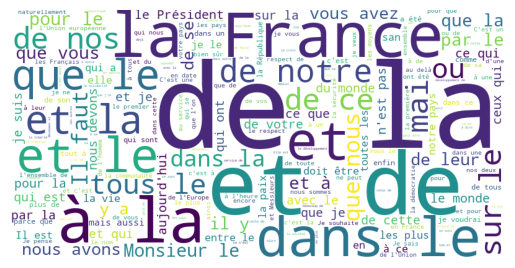
\includegraphics[width=\linewidth]{image/analyse_data/wordcloud_pres_non_pret.png}
                \caption*{\small Word cloud des discours de présidents}
            \end{minipage}\hfill
            \begin{minipage}{0.4\textwidth}
                \centering
                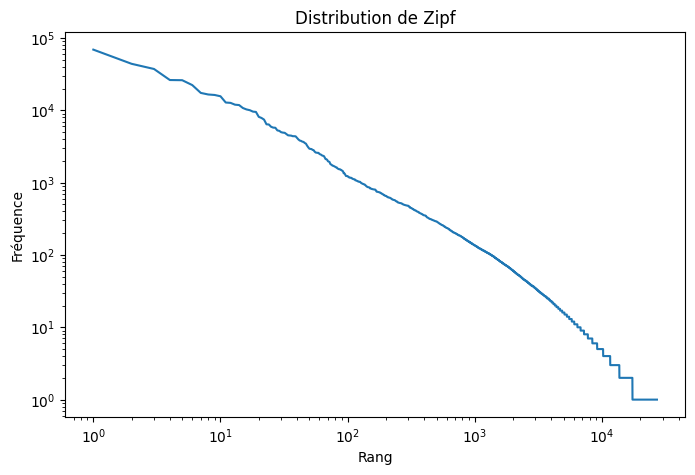
\includegraphics[width=\linewidth]{image/analyse_data/plot_zipf_pres_non_pre.png}
                \caption*{\small Distribution de Zipf des discours de présidents}
            \end{minipage}\hfill
            \label{fig:images-tests}
        \end{figure}


Comme pour les critiques de films les mots les plus fréquents sont les stops words francais.\\


\subsection{Prétraitement des données}
\subsubsection{Description}
Le prétraitement des données est une des étapes les plus importantes dans ce projet. Nous avons plusieurs techniques différentes pour faire du prétraitement pour finalement arriver à une pipeline de prétraitement qui nous semble la plus adaptée pour nos jeux de données.\\

\subsubsection{Objectifs du prétraitement}

Dans un premier temps il a fallu faire un préprétraitement des données. Nous avons d'abord converti tous les mots en minuscules afin de ne pas avoir de doublons dans notre vocabulaire. Ensuite, nous avons supprimé les caractères spéciaux et les chiffres car ils n'apportent pas d'informations pertinentes pour la classification.\\
Nous avons aussi essayé de garder uniquement les premières lignes de chaque critique de film pour voir si cela pouvait améliorer les performances de nos modèles. Cependant, cela n'a pas eu d'impact significatif sur les performances de nos modèles.\\

\subsubsection{Nettoyage du texte}

Voici une phrase en gras : \textbf{important}.

% Et en italique : \textit{remarque}.

% \section{Maths}

% Une équation simple :

% [
% a^2 + b^2 = c^2
% ]

% \section{Liste}

% \begin{itemize}
% \item Chirac
% \item Mitterrand
% \end{itemize}

\end{document}
